\documentclass{standalone}
\usepackage{tikz}
\usepackage{amsfonts}

\begin{document}
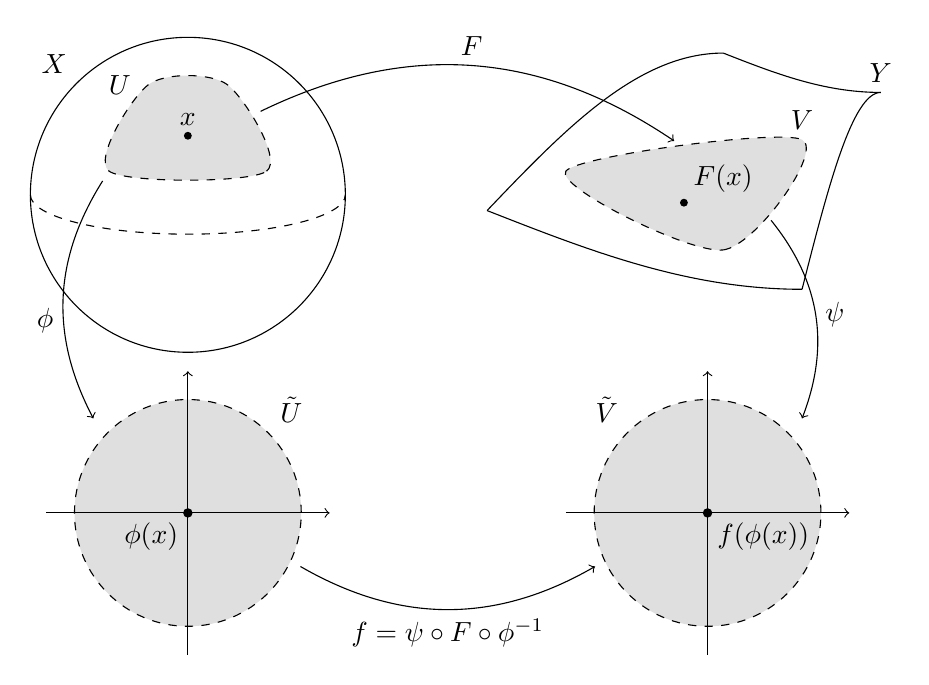
\begin{tikzpicture}
	\begin{scope}[xshift=-3cm, yshift=0.2cm]
		\draw (0,0) circle (2);
		\draw[dashed] (-2,0) arc[start angle=180, end angle=360, x radius=2, y radius=0.5];
		\draw (-{sqrt(2)}, {sqrt(2)}) node[anchor=south east]{$ X $};
		\filldraw[dashed, fill=gray!50, fill opacity=0.5] plot[smooth cycle]
		coordinates{(-1,0.3) (1,0.3) (0.5, 1.4) (-0.5, 1.4)};
		\node (x) at (0,0.75){};
		\fill (x) circle (0.05) node [above]{$ x $};
		\draw (-1,0.3) node(s1){};
		\draw (0.8,1) node(s2){};
		\node at (-0.5, 1.4) [below, left=1mm] {$ U $};
	\end{scope}

	\begin{scope}[xshift=1.8cm, yshift=0.5cm]
		\draw (-1,-0.5) node(a){};
		\draw (3,-1.5) node(b){};
		\draw (4,1) node(c){};
		\draw (2,1.5) node(d){};

		\draw (a) sin (b);
		\draw (b) sin (c);
		\draw (a) sin (d);
		\draw (d) sin (c);

		\draw (c) node[above]{$ Y $};

		\filldraw[dashed, fill=gray!50, fill opacity=0.5] plot[smooth cycle]
		coordinates{(0,0) (2,-1) (3,0.4)};
		\node at (3,0.4) [above] {$ V $};

		\node (Fx) at (1.5,-0.4){};
		\fill (Fx) circle (0.05) node [above right]{$ F(x) $};
		\draw (1.5,0.3) node(t1){};
		\draw (2.5,-0.5) node(t2){};
	\end{scope}

	\begin{scope}[scale=1.2]
		\begin{scope}[xshift=-2.5cm, yshift=-3.2cm]
			\filldraw[dashed, fill=gray!50, fill opacity=0.5] (0,0) circle (1.2);
			\draw ({sqrt(1.2)}, {sqrt(1.2)}) node{$ \tilde{U} $};
			\draw[->] (0,-1.5) -- (0,1.5);
			\draw[->] (-1.5,0) -- (1.5,0);
			\fill (0,0) circle (0.05) node[below left]{$ \phi(x) $};
			\coordinate (lc1) at (-1,1){};
			\node (lc2) at (-25:1.2){};
		\end{scope}

		\begin{scope}[xshift=3cm, yshift=-3.2cm]
			\filldraw[dashed, fill=gray!50, fill opacity=0.5] (0,0) circle (1.2);
			\draw (-{sqrt(1.2)}, {sqrt(1.2)}) node[left=-3mm]{$ \tilde{V} $};
			\draw[->] (-1.5,0) -- (1.5,0);
			\draw[->] (0,-1.5) -- (0,1.5);
			\fill (0,0) circle (0.05) node[below right]{$ f(\phi(x)) $};
			\coordinate (rc1) at (1,1){};
			\node (rc2) at (-155:1.2){};
		\end{scope}
	\end{scope}

	\draw[bend left,->] (s2) to node[above]{$ F $} (t1);
	\draw[bend right,->] (s1) to node[below left]{$ \phi $} (lc1);
	\draw[bend right, ->] (lc2) to node[below]{$ f=\psi\circ F \circ
			\phi ^{-1} $} (rc2);

	\draw[bend right, <-] (rc1) to node[right]{$ \psi $}
	(t2);
\end{tikzpicture}
\end{document}
